\chapter{Kapillarität und Auftrieb}
\label{v:3}

In diesem Versuch lernen Sie, wie man die Oberflächenspannung von Flüssigkeiten misst, sowie eine Methode zur Bestimmung der Dichte einer unbekannten Flüssigkeit.

%------------------------------------------------
\section{Stichworte}
%------------------------------------------------
Oberflächenspannung; Kapillarität; Auftrieb; Mohr'sche Waage; Drehmoment.
%
%------------------------------------------------
\section{Literatur}
%------------------------------------------------
Gehrtsen, Kapitel 3.1.4 und 3.2; Walcher, Kapitel 2.3 und 2.5
%
%------------------------------------------------
\section{Anwendungsbeispiele}
%------------------------------------------------
%
Eine Kapillare ist ein sehr feiner, langgestreckter Hohlraum. Das Wort leitet sich vom lateinischen Wort capillus (das Haar) ab.\\
Der Kapillareffekt (oder die Kapillarität) beschreibt das Verhalten einer Flüssigkeit in einer solchen Kapillare, wo die Flüssigkeit aufgrund der Oberflächenspannung an den Wänden der Kapillare ''hinaufkriecht''. Der Effekt wird zum Beispiel von Pflanzen benutzt, um Wasser von den Wurzeln, entgegen der Schwerkraft, zu den Blättern zu transportieren. In der Papierchromatographie wird eine Lösung auf Spezialpapier getropft, wo sie aufgrund der Kapillarität aufsteigt und Bestandteile der Lösung mit sich trägt. Aufgrund der Laufweiten können die Stoffe getrennt werden. Auch in Gesteinen treten Kapillareffekte auf, die Wasser durch das Gestein bewegen.
%
%------------------------------------------------
\section{Theoretischer Hintergrund}
%------------------------------------------------

\subsection{Dichtemessung}

Die Dichte eines homogenen Körpers der Masse $M$ und des Volumens $V$ ist definiert als das Verhältnis
\begin{equation} %\label{eq:Dichte}
 \rho = \frac{M}{V} \; .
\end{equation}

Die Masse eines Körpers läßt sich im Allgemeinen durch Wiegen sehr genau ermitteln. Das Volumen eines unregelmäßig geformten Körpers ist hingegen nicht einfach direkt zu bestimmen. Zur mittelbaren Bestimmung des Volumens eignet sich in vielen Fällen der Auftrieb, bzw. die Auftriebskraft $F_A$, den ein Körper erfährt, wenn man ihn in eine Flüssigkeit der Dichte $\rho_{Fl}$ taucht. Die Auftriebskraft ist gegeben durch
\begin{equation} \label{eq:Auftrieb}
 F_A = g\cdot \rho_{Fl}\cdot V\, .
\end{equation}

Hierbei ist $g$ die Erdbeschleunigung.\\
Andererseits ist die Auftriebskraft gegeben durch die Differenz der Gewichtskraft $F_g^L$, die der Körper in Luft erfährt, und der Gewichtskraft $F_g^{Fl}$, die er in der Flüssigkeit erfährt:
\begin{equation} \label{eq:Gew-Diff}
 F_A = F_g^L - F_g^{Fl} \; .
\end{equation}

Mithilfe der obigen Gleichungen findet man nun einen Ausdruck für die Dichte des Körpers:
\begin{equation} \label{eq:rho}
 \rho = \rho_{Fl}\frac{F_g^L}{F_g^L - F_g^{Fl}} \; .
\end{equation}

\subsection{Die Mohr'sche Waage}

Mißt man die Dichte eines Probekörpers zweimal nacheinander in verschiedenen Flüssigkeiten, so sind in Gleichung \ref{eq:rho} die beiden Gößen $\rho$ und $F_g^L$ konstant. Für das Verhältnis der Dichten (die \textit{relative Dichte}) ergibt sich
\begin{equation} \label{eq:rel_Dichte}
 \frac{\rho_{Fl,1}}{\rho_{Fl,2}} = \frac{F_A^{Fl,1}}{F_A^{Fl,2}} \; .
\end{equation}

Die Gewichtskräfte, die auf den Probekörper in den beiden Flüssigkeiten wirken, bestimmt man mit der Mohr'schen Waage. \\
Hierbei wird der Probekörper in Luft an die Waage gehängt, und diese über das verschiebbare Eichgewicht wieder ins Gleichgewicht gebracht. Wird der Probekörper nun in Flüssigkeit getaucht, so übt die Auftriebskraft ein Drehmoment auf den Arm der Waage aus, welches diesen nach oben drückt. Durch Auflegen der gebogenen Gewichte in die verschiedenen Positionen des Waagenarms lässt sich das Gleichgewicht wiederherstellen.\\
Damit ergibt sich:
\begin{equation}
 \rho_{Fl,1} = \rho_{Fl,2}\frac{\sum_{i=1}^n{m_i^{Fl,1}\cdot r_i}}{\sum_{j=1}^n{m_j^{Fl,2}\cdot r_j}}
\end{equation}

\subsection{Oberflächenspannung und Kapillarität}

Zwischen den Molekülen einer Flüssigkeit wirken die van~der~Waals-Kräfte. Die effektive Reichweite der van~der~Waals-Kräfte ist so klein ($F\sim r^{-6}$), daß auf ein bestimmtes Molekül in der Flüssigkeit nur die nächsten Nachbarn Kräfte ausüben. Im Inneren der Flüssigkeit sind die Moleküle homogen verteilt, sodass auf ein bestimmtes Molekül in alle Richtungen die gleiche Kraft wirkt. Diese heben sich damit auf. Die Moleküle an der Oberfläche der Flüssigkeit haben nun in einer Richtung (aus der Flüssigkeitsoberfläche hinaus) keine Nachbarn, sodass sich eine nach Innen gerichtete Gesamtkraft ergibt. Diese Kraft führt dazu, dass die Oberfläche einer Flüssigkeit dazu tendiert, eine Kugelform einzunehmen (s. Seifenblase).

Taucht man nun eine Kapillare vom Durchmesser $2r$ in eine Flüssigkeit der Dichte $\rho$, so dass sie ganz von der Flüssigkeit benetzt ist, so steigt diese in der Kapillare bis zu einer Höhe $h$ hoch. Die Flüssigkeitssäule hat die Gewichtskraft
\begin{equation}
 F_g = \rho\, V\, g = \rho\,\pi\, r^2\, h\, g
\end{equation}
und hängt an einer ringförmigen Lamelle, die die Kraft
\begin{equation}
 F_s = \sigma\, 2\,\pi\, r
\end{equation}
überträgt. Damit folgt für die Oberflächenspannung:
\begin{equation} \label{eq:Oberflaechenspannung}
 \sigma = \frac{1}{2}\rho\,g\,r\,h\; .
\end{equation}


%------------------------------------------------
\section{Fragen zur Vorbereitung}
%------------------------------------------------

\begin{enumerate} 
 \item Was soll heute im Praktikum gemessen werden? Warum?
 %
 \item Welche Kräfte wirken zwischen Molekülen in einer Flüssigkeit?
 %
 \item Was sind van der Waals-Kräfte?
 %
 \item Wodurch entsteht die Oberflächenspannung?
 %
 \item Warum erfährt ein Körper in einer Flüssigkeit Auftrieb?
 %
 \item Wie lautet das Archimedische Prinzip?
 %
 \item Warum ragt ein Eisberg aus dem Wasser?
 %
 \item Wie funktioniert die Mohr'sche Waage?
\end{enumerate} 

%------------------------------------------------
\section{Durchführung} 
%------------------------------------------------

Zu Beginn werden von der Versuchsgruppe drei verschiedene Kapillaren ausgewählt. Die Kapillare sind mit einem farbigen Rand versehen (Rot, Blau, Grün) - jede Gruppe benötigt jeweils alle drei Farben.\\

Jede der Kapillaren wird mit der Einrichtung im Raum gesäubert. Dazu gehören alle drei Stufen: 1. Lösungsmittel, 2. Weichwasser und 3. Trocknung.

\begin{enumerate}
%
 \item Messen Sie die Kapillarradien mit dem Messmikroskop: \\
 Zuerst wird die Kapillare, mit dem Ausflussende zum Experimentator zeigend, auf das Mikroskop gelegt. Dort wird durch vor-/zurückschieben der Kapillaren ein scharfes Bild eingestellt. Durch den  Schattenwurf der Kapillaren entstehen mehrere Ringe - der innerste ist hier die zu vermessende Öffnung. Das Fadenkreuz wird auf den linken Rand eingestellt und auf der Skala abgelesen. Nun wird auf den rechten Rand der Kapillaren gefahren und wiederum die Skala abgelesen. Es müssen jeweils 5 Werte aufgenommen werden.\\
 Beachten Sie: Da die Kapillaren nicht perfekt rund sind, muss die Kapillare für ein neues Wertepaar leicht gedreht werden.
 %
\end{enumerate}
%
\begin{hint}
	Da das Praktikum nur 2 Messapparate bietet, kann man sich zum Beispiel auch schon mal um die nachfolgenden Versuchsteile kümmern.
\end{hint}
\begin{figure}[ht]
	\centering
		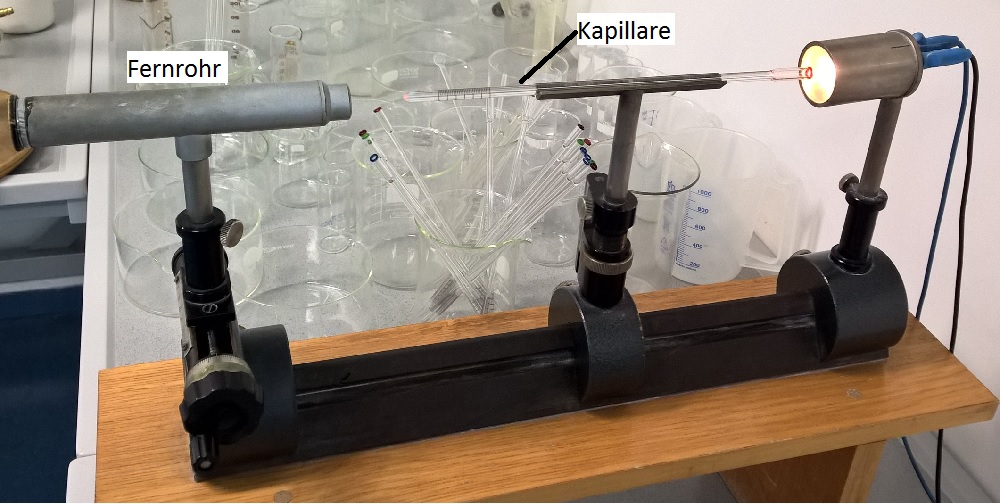
\includegraphics[width=0.7\textwidth]{Abbildungen/V7-1.jpg}
	\label{fig:V7-1}
\end{figure}

%
\begin{enumerate} \setcounter{enumi}{1}

 \begin{minipage}{0.5\textwidth}
	\item Wiegen Sie das leere Auffanggefäß und die Probekörper (jeweils einmal). 
  %
	\item Füllen Sie das Becherglas mit dem schrägen Auslass bis zu dessen Oberkante mit Wasser. Lassen Sie nun den Metallklotz in das Wasser und messen danach die Masse des Wassers im Auffanggefäß. \\
	Füllen Sie das Becherglas erneut bis zur Oberkante und lassen Sie den Holzklotz in das Wasser. Da er nicht komplett untergeht müssen Sie neben der Masse des ausgelaufenen Wassers auch die Eintauchtiefe und die Kantenlänge des Klotzes messen.
 \end{minipage}
 %
 \begin{minipage}{0.5\textwidth}
	\centering
	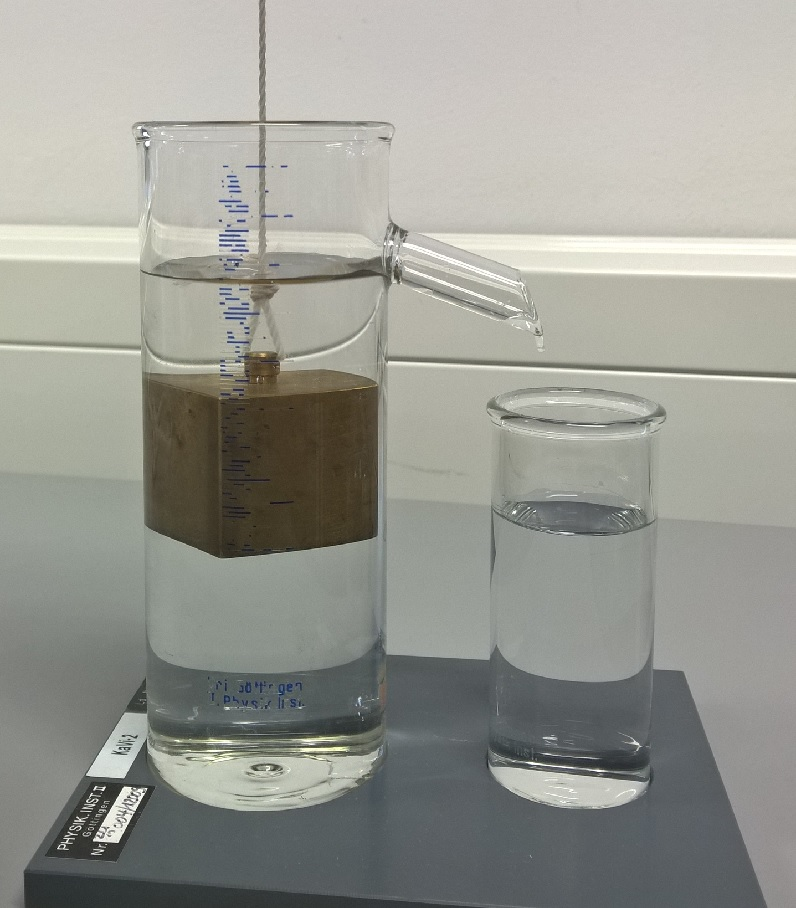
\includegraphics[width=0.7\textwidth]{Abbildungen/V7-2.jpg}
 \end{minipage}
 %
\end{enumerate}
%
\begin{hint}
	In den nachfolgenden Versuchsteilen (3 \& 4) geht es viel schneller wenn man jeweils die Versuche Steighöhen messen und Mohr'sche Waage hintereinander mit einer Flüssigkeit durchführt.
\end{hint}

Hier soll mit drei verschiedenen Flüssigkeiten gemessen werden: Wasser, Äthylenglykol, Methylalkohol. Die letzten beiden befinden sich im Eingangsbereich des Versuchsraums.
%
\begin{enumerate} \setcounter{enumi}{3}
 %
 \item Die Kapillare mit dem mittleren Radius wird tief in die Flüssigkeit getaucht. Damit ist die Innenseite der Kapillaren benetzt. Dann wird sie bis zur unteren schwarzen Markierung an der Kapillaren aus der Flüssigkeit gezogen. Hier ist die Steighöhe (innerhalb der Kapillaren) der Flüssigkeit abzulesen (1 Strich = 1 mm). Danach wird die Kapillare wieder komplett eingetaucht und erneut für eine Messung herausgezogen. Es müssen hier 5 Werte für die Steighöhe für alle 3 Flüssigkeiten bestimmt werden.
 
\begin{minipage}{0.5\textwidth}
 \item Bestimmen Sie die Dichten $\rho_{Fl}$ der drei Flüssigkeiten mithilfe der Mohr'schen Waage:
  \begin{itemize}
   \item Zuerst muss die Waage justiert werden. Dazu wird das Eichgewicht ganz langsam und vorsichtig so geschraubt, dass die Waage mit angehängtem Probekörper wieder im Gleichgewicht ist. 
   \item Danach wird der Probekörper ganz (inkl. Öse) in die zu untersuchende Flüssigkeit getaucht. Beachten Sie dabei, dass der Probekörper nicht an die Wand des Gefäßes stößt.
  \end{itemize}
\end{minipage}
%
\begin{minipage}{0.5\textwidth}
	\centering
	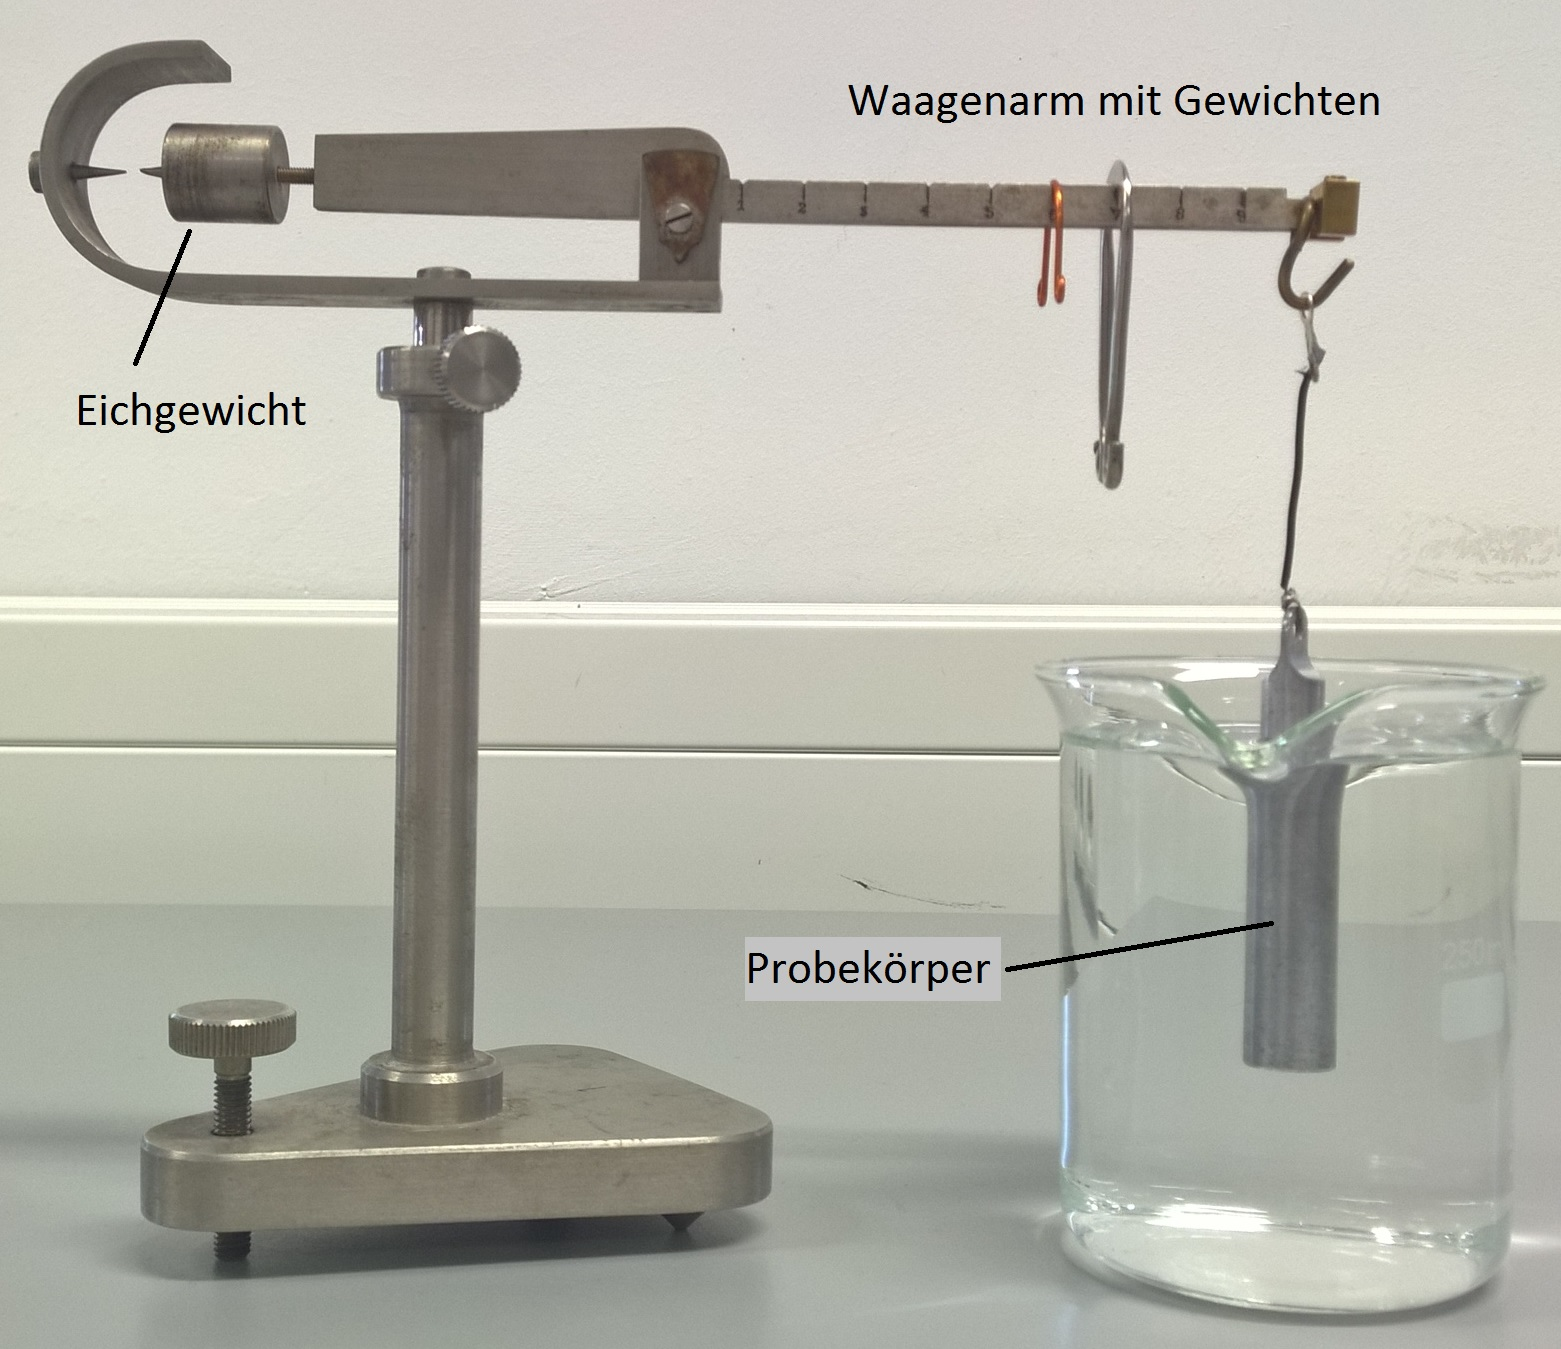
\includegraphics[width=0.8\textwidth]{Abbildungen/V7-3.jpg}
\end{minipage}

  Der Körper steigt aufgrund seines Auftriebs nach oben und bringt die Waage aus dem Gleichgewicht. Bringen Sie nun solange mit der Pinzette die gebogenen Gewichte an die verschiedenen Positionen des Waagenarms an, bis die Waage wieder im Gleichgewicht ist. Notieren Sie Lage (in cm) und Masse (in mg) der Gewichte.\\
  
  Beachten Sie, dass der Probekörper zwischen den Messungen mit verschiedenen Flüssigkeiten gründlich getrocknet werden muss. Warum?
 %
\end{enumerate}
%------------------------------------------------
\section{Auswertung} 
%------------------------------------------------
\etodo{Musterauswertung}
\begin{enumerate}
 %
 \item Bestimmen Sie die mittleren Radien $r_k$ der drei Typen von Kapillaren (blau, rot, grün) inklusive deren Fehler.
 %
 \item Berechnen Sie die Dichte $\rho_M$ des Metallkörpers inklusive Fehler.
 %
 \item Berechnen Sie die Dichte $\rho_H$ des Holzkörpers inklusive Fehler.
 %
 \item Berechnen Sie die Dichten $\rho_{Fl}$ von Äthylenglykol und Methylalkohol inklusive Fehler.
 %
 \item Bestimmen Sie die Oberflächenspannungen $\sigma$ von destilliertem Wasser, Methylalkohol und Äthylenglykol nach Gleichung \ref{eq:Oberflaechenspannung} und bestimmen Sie den Fehler von $\sigma$ aus den statistischen Messfehlern mittels Gauß'scher Fehlerfortpflanzung.
\end{enumerate}